\let\negmedspace\undefined
\let\negthickspace\undefined
\documentclass[journal]{IEEEtran}
\usepackage[a5paper, margin=10mm, onecolumn]{geometry}
%\usepackage{lmodern} % Ensure lmodern is loaded for pdflatex
\usepackage{tfrupee} % Include tfrupee package

\setlength{\headheight}{1cm} % Set the height of the header box
\setlength{\headsep}{0mm}     % Set the distance between the header box and the top of the text

\usepackage{gvv-book}
\usepackage{comment}
\usepackage{gvv}
\usepackage{cite}
\usepackage{amsmath,amssymb,amsfonts,amsthm}
\usepackage{algorithmic}
\usepackage{graphicx}
\usepackage{textcomp}
\usepackage{xcolor}
%\usepackage{txfonts}
\usepackage{listings}
\usepackage{enumitem}
\usepackage{mathtools}
\usepackage{gensymb}
\usepackage{comment}
\usepackage[breaklinks=true]{hyperref}
\usepackage{tkz-euclide} 
\usepackage{listings}
% \usepackage{gvv}                                        
\def\inputGnumericTable{}                                 
\usepackage[latin1]{inputenc}                                
\usepackage{color}                                            
\usepackage{array}                                            
\usepackage{longtable}                                       
\usepackage{calc}                                             
\usepackage{multirow}                                         
\usepackage{hhline}                                           
\usepackage{ifthen}                                           
\usepackage{lscape}
\usepackage{circuitikz}
\tikzstyle{block} = [rectangle, draw, fill=blue!20, 
    text width=4em, text centered, rounded corners, minimum height=3em]
\tikzstyle{sum} = [draw, fill=blue!10, circle, minimum size=1cm, node distance=1.5cm]
\tikzstyle{input} = [coordinate]
\tikzstyle{output} = [coordinate]


\begin{document}

\bibliographystyle{IEEEtran}
\vspace{3cm}

\title{10.3.12}
\author{EE25BTECH11013 - Bhargav}
\maketitle
    {\let\newpage\relax\maketitle}

\renewcommand{\thefigure}{\theenumi}
\renewcommand{\thetable}{\theenumi}
\setlength{\intextsep}{10pt} % Space between text and floats

\numberwithin{equation}{enumi}
\numberwithin{figure}{enumi}
\renewcommand{\thetable}{\theenumi}

\textbf{Question}: \\
If the line $y = \sqrt{3}x + K$ touches the parabola $x^2 = 16y$, then find the value of K.\\ \\
\solution \\

The equation of the conic $\brak{parabola}$ can be written as
\begin{align}
\vec{x^T}\vec{V}\vec{x} + 2\vec{u^T}\vec{x} + f = 0
\end{align}
\begin{align}
\vec{V} = \myvec{1 & 0 \\ 0 & 0}, \vec{u} = \myvec{0 \\ -8}, f=0, \vec{m^T} = \myvec{1 & \sqrt{3}}
\end{align}

\begin{align}
\vec{x} = \vec{h} + k_i\vec{m}    
\end{align}

The value of $k_i$ can be found out by solving the line and conic equation

\begin{align}
(\vec{h} + k_i \vec{m})^{\top} \vec{V} (\vec{h} + k_i \vec{m}) + 2\vec{u}^{\top} (\vec{h} + k_i \vec{m}) + f &= 0 \\
\implies k_i^{2} \vec{m}^{\top}\vec{V}\vec{m} + 2k_i \vec{m}^{\top} (\vec{V}\vec{h} + \vec{u}) + \vec{h}^{\top}\vec{V}\vec{h} + 2\vec{u}^{\top}\vec{h} + f &= 0 \\
\text{or, } k_i^{2} \vec{m}^{\top}\vec{V}\vec{m} + 2k_i \vec{m}^{\top} (\vec{V}\vec{h} + \vec{u}) + g(\vec{h}) &= 0
\end{align}

Solving the above quadratic gives the equation
\begin{align}
k_i = \frac{1}{\vec{m}^{\top}\vec{V}\vec{m}}
\brak{
    -\vec{m}^{\top} (\vec{V}\vec{h} + \vec{u})
    \;\pm\;
    \sqrt{ \sbrak{\vec{m}^{\top}(\vec{V}\vec{h} + \vec{u})}^2
    - g(\vec{h}) \, (\vec{m}^{\top}\vec{V}\vec{m}) }
    }
\end{align}

Since the tangent passes through one point of the conic, and $g\brak{\vec{q}}=0$
\begin{align}
\vec{m^T}\brak{\vec{\vec{V}\vec{q} + \vec{u}}} = 0
\end{align}
\begin{align}
\vec{m^T}\vec{V}\vec{q} = -\vec{m^T}\vec{u}
\end{align}
\begin{align}
\vec{q} = -\frac{\brak{\vec{m^T}\vec{V}}^T\vec{m^T}\vec{u}}{\norm{\vec{m^T}\vec{V}}^2}
\end{align}

On solving, we get
\begin{align}
\vec{q} = \myvec{8\sqrt{3} \\ t}, t \in \mathbf{R}
\end{align}

Since $\vec{q}$ lies on the conic, 
\begin{align}
g\brak{\vec{\vec{q}}} = 0
\end{align}
\begin{align}
\implies \vec{q^T}\vec{V}\vec{q} + 2\vec{u^T}\vec{q} + f = 0
\end{align}

Substituting and solving gives $t=12$

\begin{align}
\therefore \vec{q} = \myvec{8\sqrt{3} \\ 12}
\end{align}

Therefore $k = -12$


\begin{figure}[h!]
    \centering
    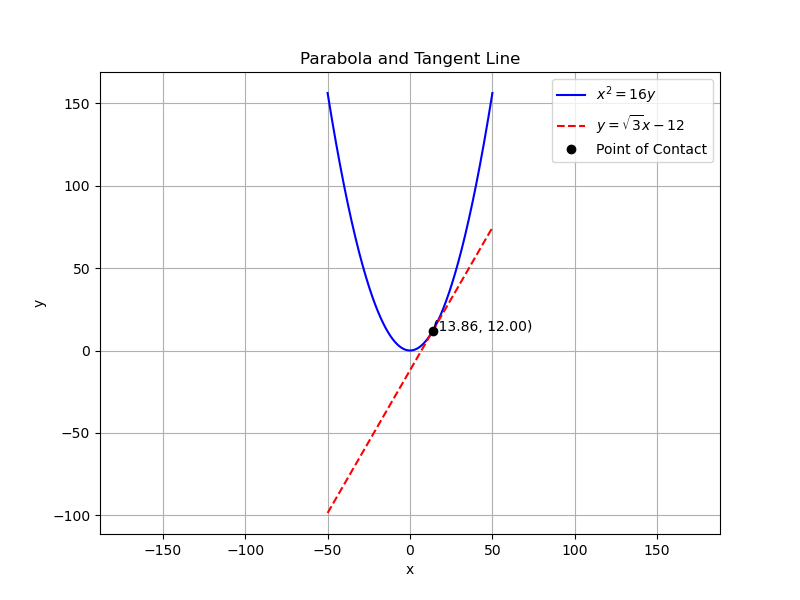
\includegraphics[height=0.5\textheight, keepaspectratio]{figs/Figure_1.png}
    \label{figure_1}
\end{figure}
\end{document}


